\chapter{Summary and conclusions}
\label{chap:conclusions}

A study of the \Hgg decay using \thisanalysislumi\ifb of $13\TeV$ data was presented, where signal-like diphoton events were sorted into orthogonal analysis categories.
Signal and background models were built from the categorised data and simulation, before undergoing statistical interpretation. The analysis differed from the official \CMS preliminary result for the same dataset~\cite{CMS-PAS-HIG-16-020} insofar as it used improvements to the parametric signal modelling and had a correction of order 6\% to the signal sample normalisation. %relating to the functional form and interpolation.

The result of the analysis is a new observation of the Higgs boson with $13\TeV$ data. The significance of the excess assuming $\mH=125.09\GeV$ is observed to be $\obsSigAtRunIBF\sigma$ ($\expSigAtRunIBF\sigma$ expected). The maximum significance is observed to be $\obsSigAtMin\sigma$ ($\expSigAtMin\sigma$ expected) for $\mH=\bestFitGlobalMH\GeV$.
Measurements of some of the properties of the observed particle were made. The best-fit global signal strength was determined to be $\obsMuBreakdown$. The best-fit fermionic and bosonic components of the signal strength were found to be $\obsMuF$ and $\obsMuV$. Furthermore, the signal strength was measured for the main Higgs boson production processes (apart from \VH), giving $\obsMuggH$, $\obsMuttH$, $\obsMuVBF$. Finally, measurements of some of the Higgs boson coupling strength modifiers were made, yielding $\obskF$ and $\obskV$ for the fermionic and bosonic modifiers and $\obskGlu$ and $\obskPho$ for the effective coupling modifiers.
All the measurements are found to be consistent with the \SM prediction within the uncertainties, which are dominated by the statistical component. 
This result is a confirmation of the Higgs boson discovery in the diphoton decay channel, using in the \RunII dataset. 
%These results show that the new particle first discovered in 2012 with the \RunI data 
The new particle behaves as predicted by the \SM for a Higgs boson at $13\TeV$. The \SM therefore continues to provide excellent agreement with data, as it has done for all measurements from collider experiments made thus far.
 
Despite its successes, however, the \SM is not a satisfactory theory to describe our universe: it is ostensibly incomplete or approximate. It does not leave room for neutrino masses which are necessary to explain the observed neutrino flavour oscillations, e.g. in~\cite{DayaBay}. The existence of dark matter cannot be explained by the \SM, and yet this is evident from, for example, the behaviour of the Bullet cluster~\cite{1538-4357-648-2-L109}. The \SM also does not account for the gravitational force or the matter-antimatter asymmetry in the universe. Furthermore, the observed mass of the Higgs boson raises the fine-tuning problem: if we assume the existence of physics beyond the \SM, radiative corrections to the Higgs boson mass should push it to the scale of new physics unless a fine-tuned cancellation occurs. Yet \mH is observed near the electroweak scale. Various extensions of the \SM seek to address these concerns. In some models the Higgs boson is a composite particle~\cite{Agashe:2004rs} or part of a wider family of Higgs bosons~\cite{Craig:2013hca}. Other theories suggest that it could be a ``portal'' to new physics~\cite{Patt:2006fw}, as it could interact with unknown particles with which regular matter cannot. All such theories would have measurable effects on the Higgs boson's production rate, interactions with other particles or multiplicity. 

In order to test some of these proposed models, refinements of the measurements presented above will become increasingly important. 
For example, the $\muttH$ parameter is sensitive to additional top-like particles, which have been proposed to resolve the fine-tuning problem. Such additional particles are also predicted by many theories which address neutrino oscillations, dark matter, and matter-antimatter asymmetry, for example supersymmetry~\cite{Martin:1997ns}.  
As presented above, the rate of $ttH (\gamma \gamma)$ is consistent with the \SM, but with $\sim$150\% uncertainty. Evidently, there is plenty of room for discrepancies to hide within the current measurements. Recent extrapolations of the \CMS results shown in \Fig~\ref{fig:conc:extrapolations}, which the author was responsible for producing, showed that reducing these uncertainties to the $\sim$30\% level could be achievable in the next five years, and down to the $\sim$15\% by the end of the LHC programme~\cite{CMS-DP-2016-064}. Such improvements will put stringent constraints on the nature of physics beyond the \SM, particularly when combined with results from other decay channels. 
\begin{figure}[ht!]
\centering
\subfloat[]{
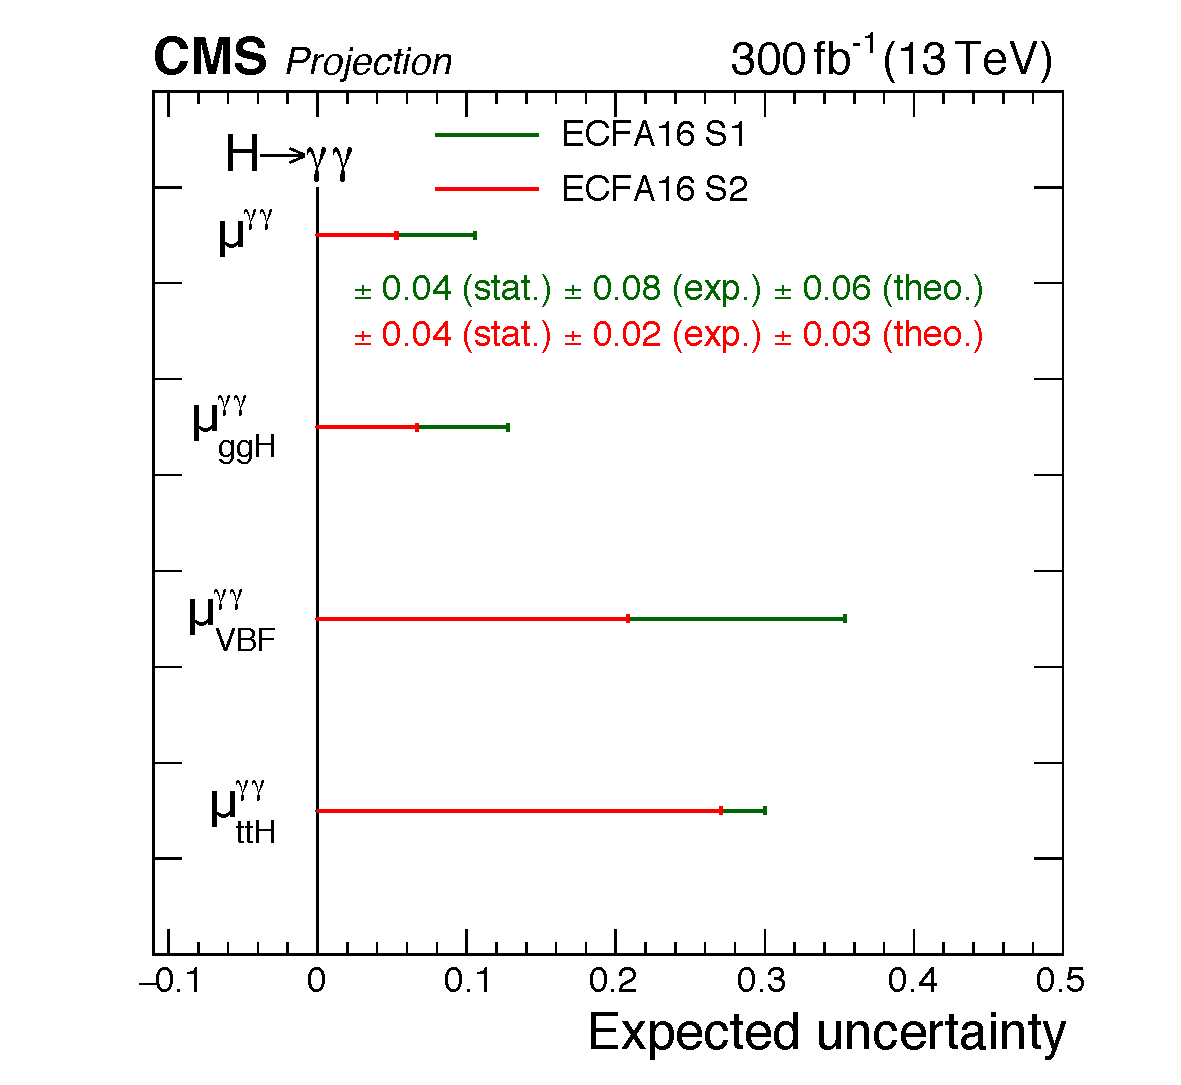
\includegraphics[width=0.6\textwidth]{conclusionFigures/new_mu_plot_300.pdf}}\\
\subfloat[]{
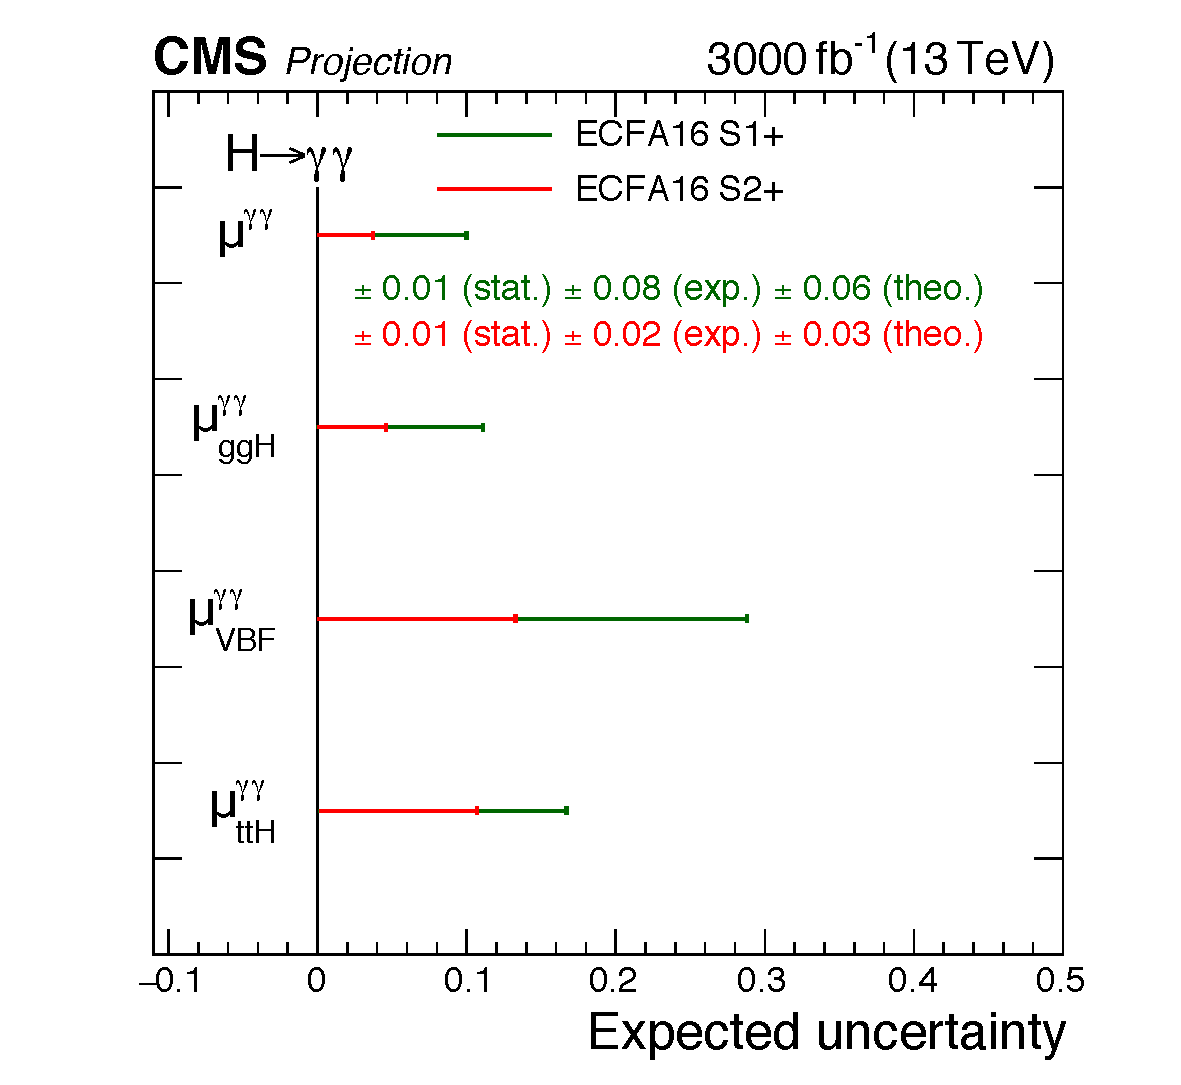
\includegraphics[width=0.6\textwidth]{conclusionFigures/new_mu_plot.pdf}}
\caption[Projections for the uncertainties on signal strength measurements using the \Hgg decay, assuming (a) 300\ifb and (b) 3000\ifb have been collected. In scenario S1, all systematic uncertainties are kept constant and only statistical uncertainties are reduced. In scenario S2, the experimental systematic uncertainties are reduced with the square root of the integrated luminosity (until a lower threshold based on achievable detector accuracy is reached), while the theoretical systematic uncertainties are reduced by a factor of 2. The "+" indicates that the effects of increased \PU and planned detector upgrades are accounted for\quad\cite{CMS-DP-2016-064}.]{Projections for the uncertainties on signal strength measurements using the \Hgg decay, assuming (a) 300\ifb and (b) 3000\ifb have been collected. In scenario S1, all systematic uncertainties are kept constant and only statistical uncertainties are reduced. In scenario S2, the experimental systematic uncertainties are reduced with the square root of the integrated luminosity (until a lower threshold based on achievable detector accuracy is reached), while the theoretical systematic uncertainties are reduced by a factor of 2. The "+" indicates that the effects of increased \PU and planned detector upgrades are accounted for~\cite{CMS-DP-2016-064}.}
\label{fig:conc:extrapolations}
\end{figure}

The field of Higgs physics therefore finds itself in a new and exciting situation. The discovery of the Higgs boson has opened a new avenue with which to study fundamental questions about our universe. This avenue will be exploited for the very first time in the coming decade, as the field pivots from the discovery era into the precision measurement era. Future studies of the Higgs boson's properties will either set strong limits on proposed theories or reveal clues to new physics beyond the \SM. 

